\section{Experiments}
\label{sec:exp}
We conduct experiments to investigate the performance of the proposed MTSL 
methods. As has been said above, our experiments are conducted on the 
proposed \textbf{L}arge-scale \textbf{R}eal-world \textbf{O}rder 
\textbf{D}ataset (LROD). \KZ{I'm not sure if reader will be confused by
the word ``order''.. Maybe say transaction order?}

\subsection{Data Collection}
\label{sec:data}
To the best of our knowledge, available large scale real-world order dataset is very rare, especially with real-sized items. For that purpose, we create a dataset on 3D flexible bin packing problem of real-world E-commerce platform. This LROD consists of two parts: the customer order data is collected from E-commerce platform and item size data (i.e., length, width and height) is collected from Logistics platform. We randomly sample 150,000 training data and 150,000 testing data for customer orders with 8, 10 and 12 items, which are named as BIN8, BIN10 and BIN12 respectively. This dataset can be used to solve our 3D-FBPP as well as other applications, such as box design. We believe this dataset will contribute to the future research of 3D packing problem. \footnote{The data will be published soon after accepted.}
\KZ{How do you know the packing data you obtained is optimal and can be used
for training? I know humans are good, but if human workers are so good at
packing, what's the point of this paper?}

\subsection{Implementation Details}
\label{sec:implementation}
Across all experiments, we use mini-batches of 128 problems, LSTM cells with 128 hidden units, and embed the three coordinates of each item in a 256-dimensional space. We train our model with Adam optimizer \cite{kingma2014adam} with initial learning rate of $10^{-3}$ and decay every 5000 steps by a factor of 0.96. All the parameters are initialized randomly in $[-0.08,0.08]$ and clip $L2$ norm of our gradients to 5.0. We initialized the surface area baseline by LWSC and resort an exponential moving average  baseline with decay factor $\alpha=0.7$. We use 1000,000 steps to train the model and it will take about 70 hours on Tesla M40 GPU machine. Model implementation with TensorFlow will be made available soon.
Based on comprehensive consideration, the performance indicator is average surface area (ASA) which denotes the average cost of packing materials. The mathematical definition of ASA is as follows:
\begin{eqnarray*}
	ASA = \frac{\sum_{i=1}^{n} SA(i)}{n},
\end{eqnarray*}
where $SA(i)$ is the surface area of $i$th order and $n$ is the number of order.

We will show the detailed experimental and comparison procedures in the follows.


\subsubsection{Multi-task Selected Learning Training}

For MTSL experiments, at each step, we choose a loss function of $\{L_{seq}, L_{ori}, L_{all}\}$ defined in \secref{sec:train} at each batch adapting to the training process. Actually, we sample these three losses with probabilities $(0.3, 0.5, 0.2)$. The values of probabilities are annealed to $(0.33, 0.33, 0.33)$ respectively over the first 10,000 training steps. Furthermore, we sample 800 times for each test instance and obtain the best as described in \secref{sec:test}. 
For comparison, we computed three kinds of ASA: 1) the sequence is generated by the sequence task of MTSL model and orientation is generated according to LWSC; 2) the sequence and orientation are both generated by our MTSL model; 3) the sequence is generated by the sequence task of MTSL model and orientation is randomly generated. We refer to those results as MTSL-ST-sample, MTSL-MT-sample and MTSL-Rand-sample to verify the effectiveness of probability distribution of orientations calculated by our MTSL model. Besides, we also conduct an experiment without Selected Learning called MT-sample, whose loss function is $L_{all}$.

\subsubsection{Reinforcement Learning Training}
In addition to the described methods, we also implement and train a pointer network with reinforcement learning as the strong baseline method. It's a single task model and
the stochastic policy of this RL model is only related to the sequence of placing the items into bin, since other major factors are defined by LWSC mentioned above.
%Previous work has already proved the effectiveness of this method against the heuristic method, in which experiments shows that the reinforcement learning results with beam search at inference time are better than the NBPH baseline with an improvement of about $4.8\%$ \cite{Hu2017Solving}.
We refer it as RL-vanilla in our paper. However, the vanilla method never takes the packing sequence that has already been produced into consideration.
We will empirically show the necessity of the introduced intra-attention mechanism through plenty of experiments and we refer this as RL-intra.
Consequently, the remaining experiments about RL models have introduced the intra-attention mechanism by default.
Furthermore, in order to carry out comparative test with the MTSL model, as our MTSL model adopts sampling strategy to obtain the best result at inference time, we also apply it in RL model. We call this approach RL-intra-sample. %Meanwhile, to verify the effectiveness of probability distribution of orientations calculated by our MTSL model, we compare the results of the sequence generated by RL model following by random orientations, which is denoted as RL-multiple-sample. %We refer to those approaches as RL vanilla-bs, RL intra-bs, RL single-sample and RL multiple-sample. \yu{I cannot distinguish them, maybe point out directly.}

%\noindent
\subsection{Results and Analysis}
\label{sec:eval}
First of all, we evaluate different models including RL-vanilla and RL-intra on our proposed dataset LORD. We report the ASA in Table \ref{rl-result}. As the table shows, the RL-vanilla achieves $4.89\%$, $4.88\%$, $5.33\%$ improvement than LWSC for BIN8, BIN10 and BIN12, whereas the improvement of the RL-intra is increased to $5.19\%$, $5.26\%$, $5.41\%$ instead. Apparently, this demonstrates the usefulness of our intra-attention training method for the 3D-FBPP which can help reduce the surface area. 
Besides, we also conduct the approach BRKGA in \cite{gonccalves2013biased} on LORD to validate whether these method designed for fixed-sized bin are appropriate for our 3D-FBPP. BRKGA is one of the state-of-the-art method to tackle 2D and 3D fixed-sized bin packing problems which adopts a heuristic method of Genetic Algorithm. According to Table \ref{rl-result}, we find that BRKGA is dramatically limited by the non-fixed-sized bin. It even performs worse than the random method which randomly generates the packing sequence and adopts the orientation and spatial location calculated by LWSC. All in all, the statistical analysis confirms that RL intra-bs is significantly better than all the other approaches outlined below.
\begin{table}[!htb]
	\vspace{-10pt}
	\centering
	\begin{tabular}{l|l l l}
		\hline
		model &   BIN8 & BIN10 & BIN12 \\ \hline
		Random &  44.70 & 48.38 & 50.78 \\ 
		LWSC & 43.97 & 47.33 & 49.34 \\
		BRKGA  &59.44 & 65.73 & 68.47 \\
		RL-vanilla & 41.82 & 45.02 & 46.70 \\ 
		RL-intra & \textbf{41.69} & \textbf{44.84} & \textbf{46.67} \\ \hline
	\end{tabular}
    \caption{ASA Comparison of RL-vanilla and RL-intra on the LORD.}
    \label{rl-result}
	\vspace{-10pt}
\end{table}
\KZ{Why not combine Table 1 and 2?}
Thus, we report the ASA of our remaining approaches on BIN8, BIN10, and BIN12 in Table \ref{bin result}. Notably, results demonstrate that training with RL and MTSL significantly comfortably surpass the LWSC. By calculation, the proposed MTSL-MT-sample achieves $6.21\%$, $7.80\%$, $8.55\%$ improvement than the greedy LWSC for BIN8, BIN10, and BIN12. In our experiments, MTSL-MT-sample proves superior than other methods in most cases but is slightly less competitive than RL-intra-sample in BIN8. The comparison between MT-sample and MTSL-MT-sample also indicates the effectiveness of Selected Learning. Without Selected Learning, the multi-task method performs much worse than the single task method RL-intra-sample. Furthermore, these results also illustrate that multi-task selected learning model always get more competitive result than the single task RL model and the MTSL is significantly meaningful for problem like the 3D-FBPP.
\begin{table}[!htb]
	\centering
	\begin{tabular}{l|l l l}
		\hline
		model &   BIN8 & BIN10 & BIN12 \\ \hline
		Random &  44.70 & 48.38 & 50.78 \\ 
		LWSC & 43.97 & 47.33 & 49.34 \\ 
		MTSL-ST-sample & 42.25 & 44.34 & 45.30 \\ 
		MTSL-MT-sample & 41.24 & \textbf{43.64} & \textbf{45.12} \\ 
		MTSL-Rand-sample & 42.21 & 44.41 & 45.42 \\ 
		RL-intra-sample & \textbf{41.12} & 44.03 & 45.58 \\ 
		MT-sample & 42.31 & 46.01 & 47.32 \\ \hline
	\end{tabular}
	\caption{ASA of mentioned methods, and all ASA are obtained of 800 times sampling. }
	\label{bin result}
	\vspace{-10pt}
\end{table}

We present a more detailed comparison of our methods in Figure \ref{fig:curve-model}, where we show the relationship between their performances and corresponding sampling times. The curve reveals a fact that MTSL-MT-sample approach which produces the sequence and orientations simultaneously outperforms other learning configurations in most cases. The contrast between MTSL methods demonstrate that the probability distribution of orientations calculated by our MTSL model is indeed effective, as the ASA with MTSL-MT-sample significantly improves over MTSL-ST-sample and MTSL-Rand-sample. Furthermore, we find that the orientation task can definitely promote better results, even though the MTSL-MT-sample is just a few percents worse than greedy LWSC baseline and MTSL-ST-sample at the very beginning. Moreover, MTSL-MT-sample approach benefits from much less orientation search space and run efficient than the methods that adopt the LWSC to calculate orientation which will search from $6^n$ space at most.
%\begin{figure}[h]
%	\centering
%	\subfigure[]{\includegraphics[width=0.49\columnwidth]{figure/BIN8.pdf}} \hfill
%	\subfigure[]{\includegraphics[width=0.49\columnwidth]{figure/BIN10.pdf}}\\
%	\subfigure[]{\includegraphics[width=0.49\columnwidth]{figure/BIN12.pdf}}
%	\caption{Results for multi-task binpacking network. (a), (b), (c) shows the result of BIN8, BIN10, BIN12, respectively.}
%	\label{fig:curve-model}
%	\vspace{-10pt}
%\end{figure}
%

\begin{figure*}[th]
	\centering
	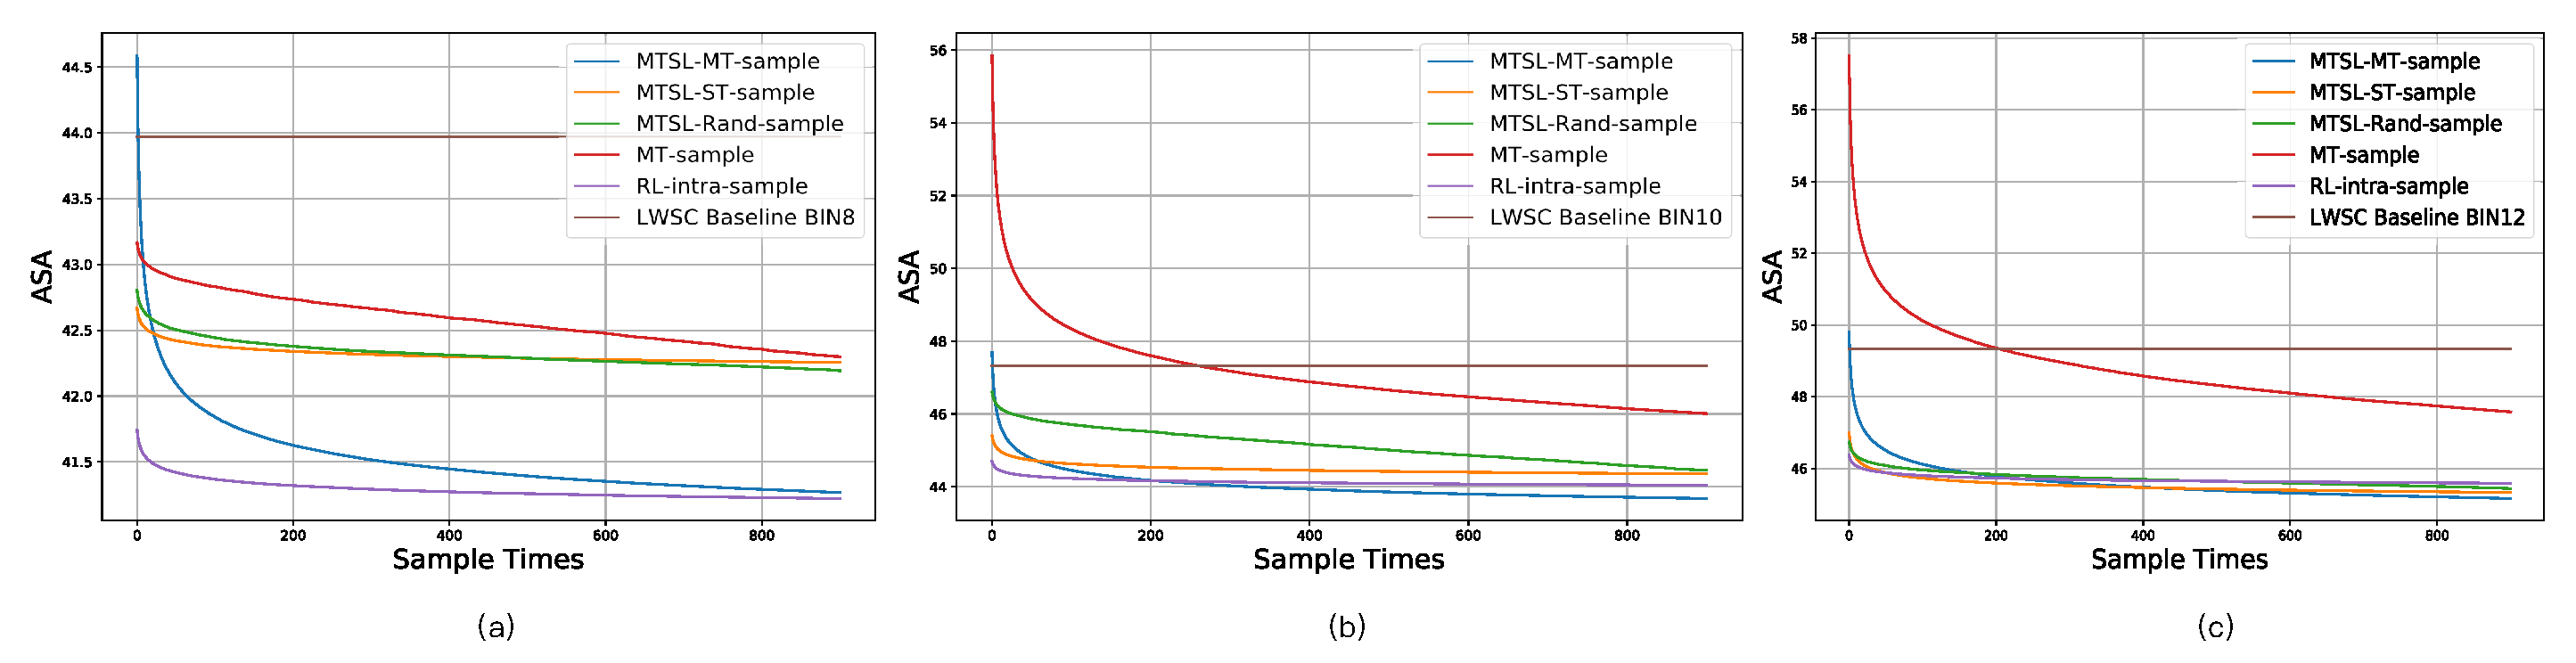
\epsfig{file=binresult.eps, width=2.0\columnwidth}
	\caption{Results for multi-task binpacking network. (a), (b), (c) shows the result of BIN8, BIN10, BIN12, respectively.}
	\label{fig:curve-model}
	\vspace{-10pt}
\end{figure*}

Finally, we randomly pick an example order and produce results by different methods in Figure \ref{fig:result-example} for case study. The example order is from BIN8 and the results are obtained by sampling 500 times.
As shown, the surface area computed by each method is listed on the top of each results. Obviously, the computational experiment results demonstrate that MTSL-MT-sample can produce a more reasonable packing policy than other methods. 

%\begin{figure}[h]
%	\centering
%\subfigure[SL %single-sample]{\includegraphics[width=0.48\columnwidth]{figure/SL-single-sample.pdf}} \hfill
%\subfigure[SL multiple-sample]{\includegraphics[width=0.48\columnwidth]{figure/SL-multiple-sample.pdf}}\\
%\subfigure[RL single-sample]{\includegraphics[width=0.48\columnwidth]{figure/RL-single-sample.pdf}}\hfill
%\subfigure[RL multiple-sample]{\includegraphics[width=0.48\columnwidth]{figure/RL-multiple-sample.pdf}}\\
%\subfigure[NBPH Method]{\includegraphics[width=0.48\columnwidth]{figure/NBPH			Method.pdf}}
%	\caption{Sampled result of bpp. NBPH method result and SL single-sample, SL multiple-sample, RL single-sample, RL multiple-sample.}
%	\label{fig:result-example}
%	\vspace{-10pt}
%\end{figure}

\begin{figure}[h]
	\vspace{-10pt}
	\centering
	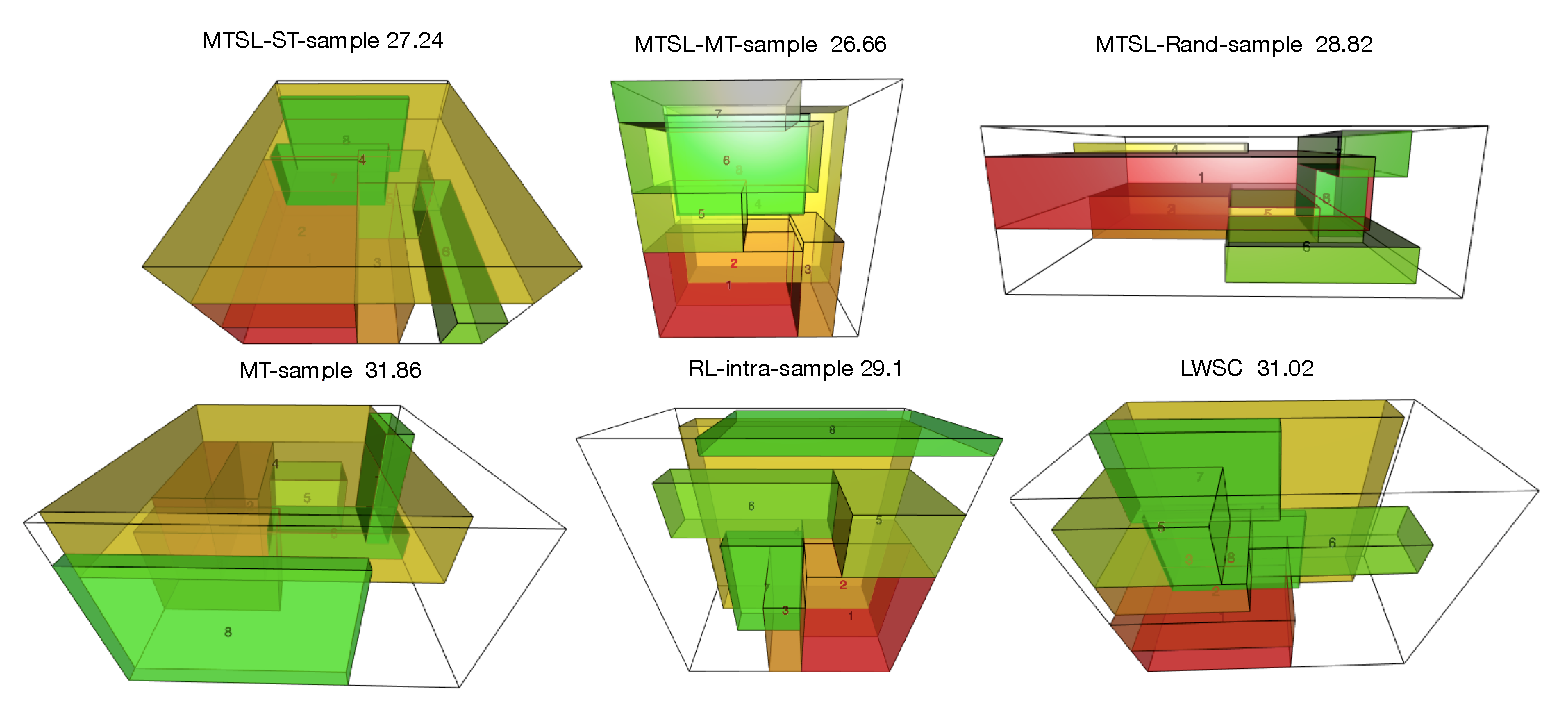
\epsfig{file=binpackingresult.eps, width=0.95\columnwidth}
	\caption{Results of MTSL-ST-sample, MTSL-MT-sample, MT-Rand-sample, MT-sample,RL-intra-sample and LWSC. The surface area of these method are 27.24, 26.66, 28.82, 31.86, 29.1 and 31.02 respectively}
	\label{fig:result-example}
	\vspace{-10pt}
\end{figure}
